\section{Ações de Engastamento}

No caso de um carregamento genérico atuando no plano do elemento, como mostrado na figura~\ref{fig:el-acao-carregamento-generico}, que pode ser decomposto em uma componente normal ($q_2$) e outra tangencial ($q_1$), as ações de extremidade de elemento também podem ser determinadas pelas equações~\ref{eq:caso1-Aii} ou~\ref{eq:caso2-Aff}, impondo-se a condição de que os nós do elemento são restringidos, isto é, fazendo-se $\mathbf{u}_I = \mathbf{u}_F = 0$. Escolhendo-se o sistema de equações~\ref{eq:caso1-Aii}, que corresponde ao sistema principal mostrado na figura~\ref{fig:casos-considerados}, segue:
\begin{equation}
	\begin{bmatrix}
		\mathbf{E}_{II} & \mathbf{E}_{IF} \\
		\mathbf{A}_{II} & \mathbf{0}
	\end{bmatrix}
	\times
	\begin{bmatrix}
		\mathbf{f}_{I0} \\
		\mathbf{f}_{F0}
	\end{bmatrix}
	=
	\begin{bmatrix}
		-\mathbf{F}_0 \\
		\mathbf{u}_{I0}
	\end{bmatrix},
\end{equation}

onde $\mathbf{f}_{I0}$ e $\mathbf{f}_{F0}$ são as ações de extremidade de elemento devidas a carga de membro, e $\mathbf{u}_{I0}$ é dado pela equação~\ref{eq:Aii}.

\begin{figure}[!htbp]
	\centering
	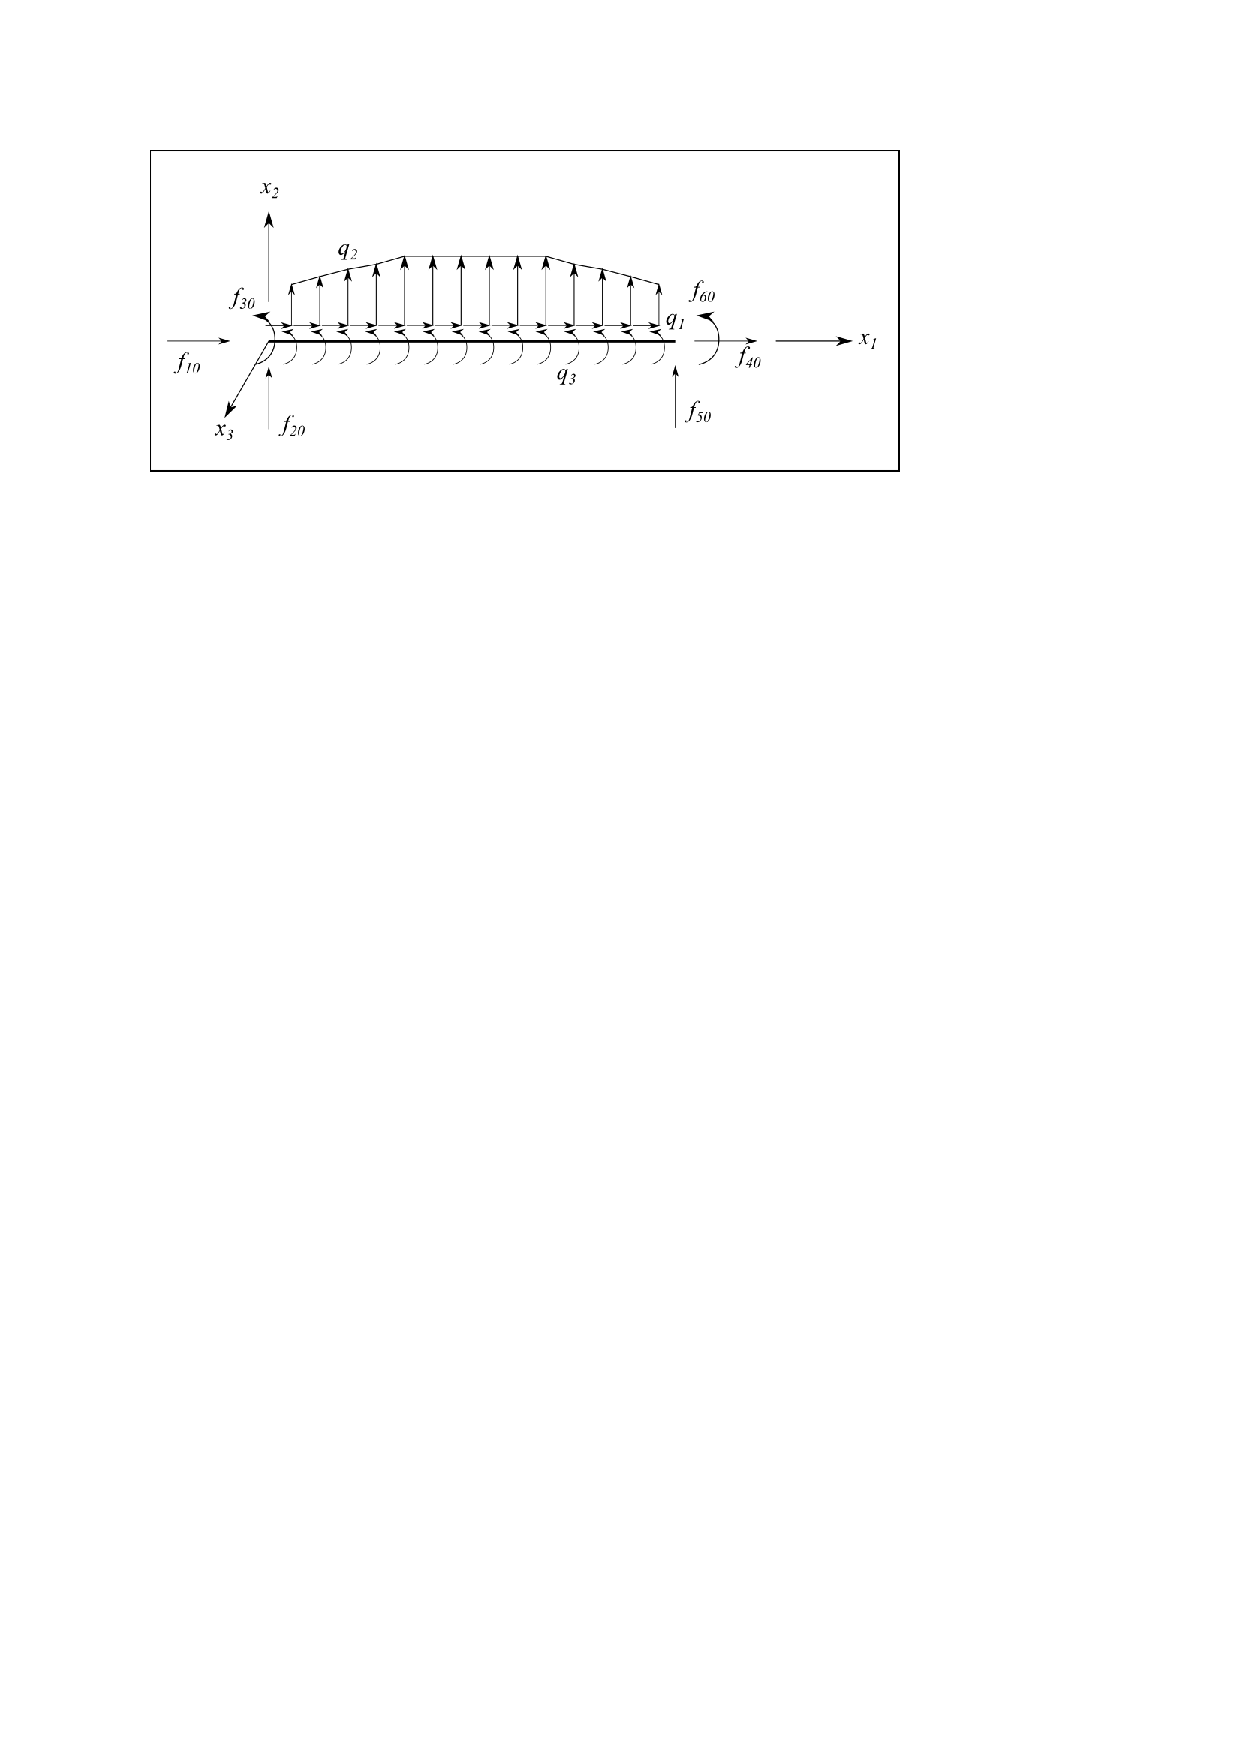
\includegraphics[trim = 30mm 220mm 60mm 29mm, clip, scale=1.1]{img/el-acao-carregamento-generico.pdf}
	\caption{Elemento sob a ação de carregamento genérico}
	\label{fig:el-acao-carregamento-generico}
\end{figure}

Neste artigo, utiliza-se uma função de interpolação quadrática para aproximar a carga no elemento, de modo que conhecendo-se os valores da função de carga, no início ($x_1=0$), no meio ($x_1=\dfrac{l}{2}$), e no fim ($x_1=l$) do elemento, respectivamente, as correspondentes expressões aproximadas para as funções de carga e esforços internos, $^{(m)}M_0 = M(q_2,q_3),\, ^{(m)}Q_0 = Q(q_2),\, ^{(m)}N_0 = N(q_1)$ podem ser determinadas. Resulta, para $m=1$:
\begin{align}
	^{(1)}u_{10}
	 & = -\int_l \dfrac{^{(1)}N_q(x'_1)}{k_a}\,dx'_1;\, ^{(1)}u_{20} = \int_l \left( \dfrac{x_1\,^{(1)}M_q(x'_1)}{k_b} + \dfrac{^{(1)}Q_q(x'_1)}{k_s}\right)\,dx'_1;\, \nonumber \\
	^{(1)}u_{30}
	 & = -\int_l \dfrac{^{(1)}M_q(x'_1)}{k_b}\,dx'_1.\,
\end{align}

onde

\begin{align}
	^{(1)}N_q(x_1)
	 & = \sum_{k=1}^3\, ^{(1)}N_{q_k}(x'_1) = \,^{(1)}N_{q_1}(x'_1)                       \nonumber   \\
	^{(1)}M_q(x_1)
	 & = \sum_{k=1}^3\, ^{(1)}M_{q_k}(x'_1) = \,^{(1)}M_{q_2}(x'_1) + \,^{(1)}M_{q_3}(x'_1) \nonumber \\
	^{(1)}Q_q(x_1)
	 & = \sum_{k=1}^3\, ^{(1)}Q_{q_k}(x'_1) = \,^{(1)}Q_{q_2}(x'_1)
\end{align}

\begin{align}
	^{(1)}N_q(x_1)
	 & = -\int_0^{x_1} q_1(\xi)d\xi = -a_1 \dfrac{x_1^3}{3} - b_1 \dfrac{x_1^2}{2} - c_1x_1,                                                \\
	^{(1)}Q_q(x_1)
	 & = \int_0^{x_1} q_2(\xi)d\xi = a_2 \dfrac{x_1^3}{3} + b_2 \dfrac{x_1^2}{2} + c_2 x_1,                                                 \\
	^{(1)}M_q(x_1)
	 & = \int_0^{x_1} (x_1-\xi)q_2(\xi) - q_3(\xi)d\xi = \dfrac{1}{12}a_2x_1^4 + \dfrac{1}{6}b_2x_1^3 + \dfrac{1}{2}c_2x_1^2 - \, \nonumber \\
	 & -\dfrac{1}{3}a_3x_1^3 - \dfrac{1}{2} b_3x_1^2 - c_3x_1,
\end{align}

com

\begin{align}
	a_k & = -\dfrac{2}{l^2}(2q_{k2} - q_{k1} - q_{k3}), k=1,2,3, \\
	b_k & = \dfrac{1}{l}(4q_{k2} - 3q_{k1} - q_{k3}), k=1,2,3,   \\
	c_k & = q_{k1}, \quad k=1,2,3 \;,
\end{align}

\noindent $q_{ki}$ sendo o valor da \textit{k}-ésima componente da taxa de carga distribuída, $q_k$, no \textit{i}-ésimo nó do elemento.
Para $m=2$, tem-se:

\begin{equation}
	^{(2)}u_{40} = \int_l \dfrac{^{(2)}N_q}{k_a}\,
	dx'_1,\, \quad
	^{(2)}u_{50} = \int_l \left( \dfrac{(l-x_1)\, ^{(2)}M_q}{k_b} + \dfrac{^{(2)}Q_q}{k_s}\right)\, dx'_1,\, \quad
	^{(2)}u_{60} = \int_l \dfrac{^{(2)}M_q}{k_b}\,dx'_1.\,
\end{equation}

onde

\begin{align}
^{(2)}N_q(x_1)       & = \sum_{k=4}^6\, ^{(2)}N_{q_k} \nonumber \\
                    ^{(2)}M_q(x_1) & = \sum_{k=4}^6\, ^{(2)}M_{q_k} \nonumber \\
                    ^{(2)}Q_q(x_1) & = \sum_{k=4}^6\, ^{(2)}Q_{q_k}
\end{align}

\begin{align}
^{(2)}N_q(x_1)       & = \int_0^{x_1} q_1(\xi)d\xi,                     \\
                    ^{(2)}Q_q(x_1) & = -\int_0^{x_1} q_2(\xi)d\xi,                    \\
                    ^{(2)}M_q(x_1) & = \int_0^{x_1} q_3(\xi) + (\xi-x_1)q_2(\xi)d\xi,
\end{align}

A expressão $\mathbf{u}_{I0}$ de é também avaliada numericamente pela quadratura Gaussiana através da expressão abaixo:
\begin{equation}
	u_{i0}
	=
	\int_l g_i(x_1)\,dx_1
	=
	\dfrac{l}{2} \sum_{k=1}^{\textrm{npg}} g_i[x_1(\eta_k)]\omega_k, \quad
	i=1,2,3.
\end{equation}

onde $g_i$ é o correspondente integrando dado na equação~\ref{eq:gauss-legendre}.